\documentclass{article}
\usepackage[left=2cm, right=2cm, top=0cm]{geometry}
\usepackage{amsmath}
\usepackage{amssymb}
\usepackage{fancyvrb}
\usepackage{xcolor}

\usepackage{graphicx}
\usepackage{enumitem}
\usepackage{tikz}
\usepackage{pgfplots}
\usepackage{pdflscape}
\usepackage{fancyhdr} 

\fancypagestyle{mylandscape}{
\fancyhf{} %Clears the header/footer
\fancyfoot{% Footer
\makebox[\textwidth][r]{% Right
  \rlap{\hspace{.75cm}% Push out of margin by \footskip
    \smash{% Remove vertical height
      \raisebox{4.87in}{% Raise vertically
        \rotatebox{90}{\thepage}}}}}}% Rotate counter-clockwise
\renewcommand{\headrulewidth}{0pt}% No header rule
\renewcommand{\footrulewidth}{0pt}% No footer rule
}


\usepackage{hyperref}
\setlength\parindent{0pt}
% \hypersetup{
%    colorlinks,
%    citecolor=green,
%    filecolor=black,
%    linkcolor=blue,
%    urlcolor=blue
%}
\begin{document}
\title{Homework 1: Population Survey}
\author{Jacob Puthipiroj}
%\date{}
\maketitle


The Current Population Survey refers to any of the monthly surveys conducted by the US Census Bureau throughout the year, although the March CPS --considered the beginning of the annual survey cycle-- is the most significant, and is the data used in this assignment. Broadly, the CPS collects cross-sectional employment data of the participating households, allowing for regression wherein the independent and dependent variables are associated with the same point in time. In this assignment, I explore the relationship between educational attainment on earnings, parameterized as follows:

\begin{itemize}
\item Independent variable: $a\_hga$, an ordinal categorical variable denoting various levels of educational attainment, from the completion of less than 1st grade, to those who complete a PhD.
\item Dependent variable: $ptot\_r$, an ordinal categorical variable denoting 41 levels of personal income. Variables are topcoded: rounded up to the nearest \$2,500. Thus the first level includes all incomes from \$0-\$2,500, while the last level includes all incomes above \$100,000. Such discretization allows for easier data collection, but involves loss of information and introduces an upward bias in recorded incomes, up until \$100,000, where it does not make further distinctions and instead reduces a downward bias.\footnote{\#data: I give background context for the CPS Survey, explaining the sample and methodology, and explain in detail the data structure of the two variables involved: Educational Attainment (ordinal categorical), and Personal Income (originally continuous, discretized into 41 ordinal categories of width \$,2500 each). }

\end{itemize}





\begin{figure*}[h]
	\centering
	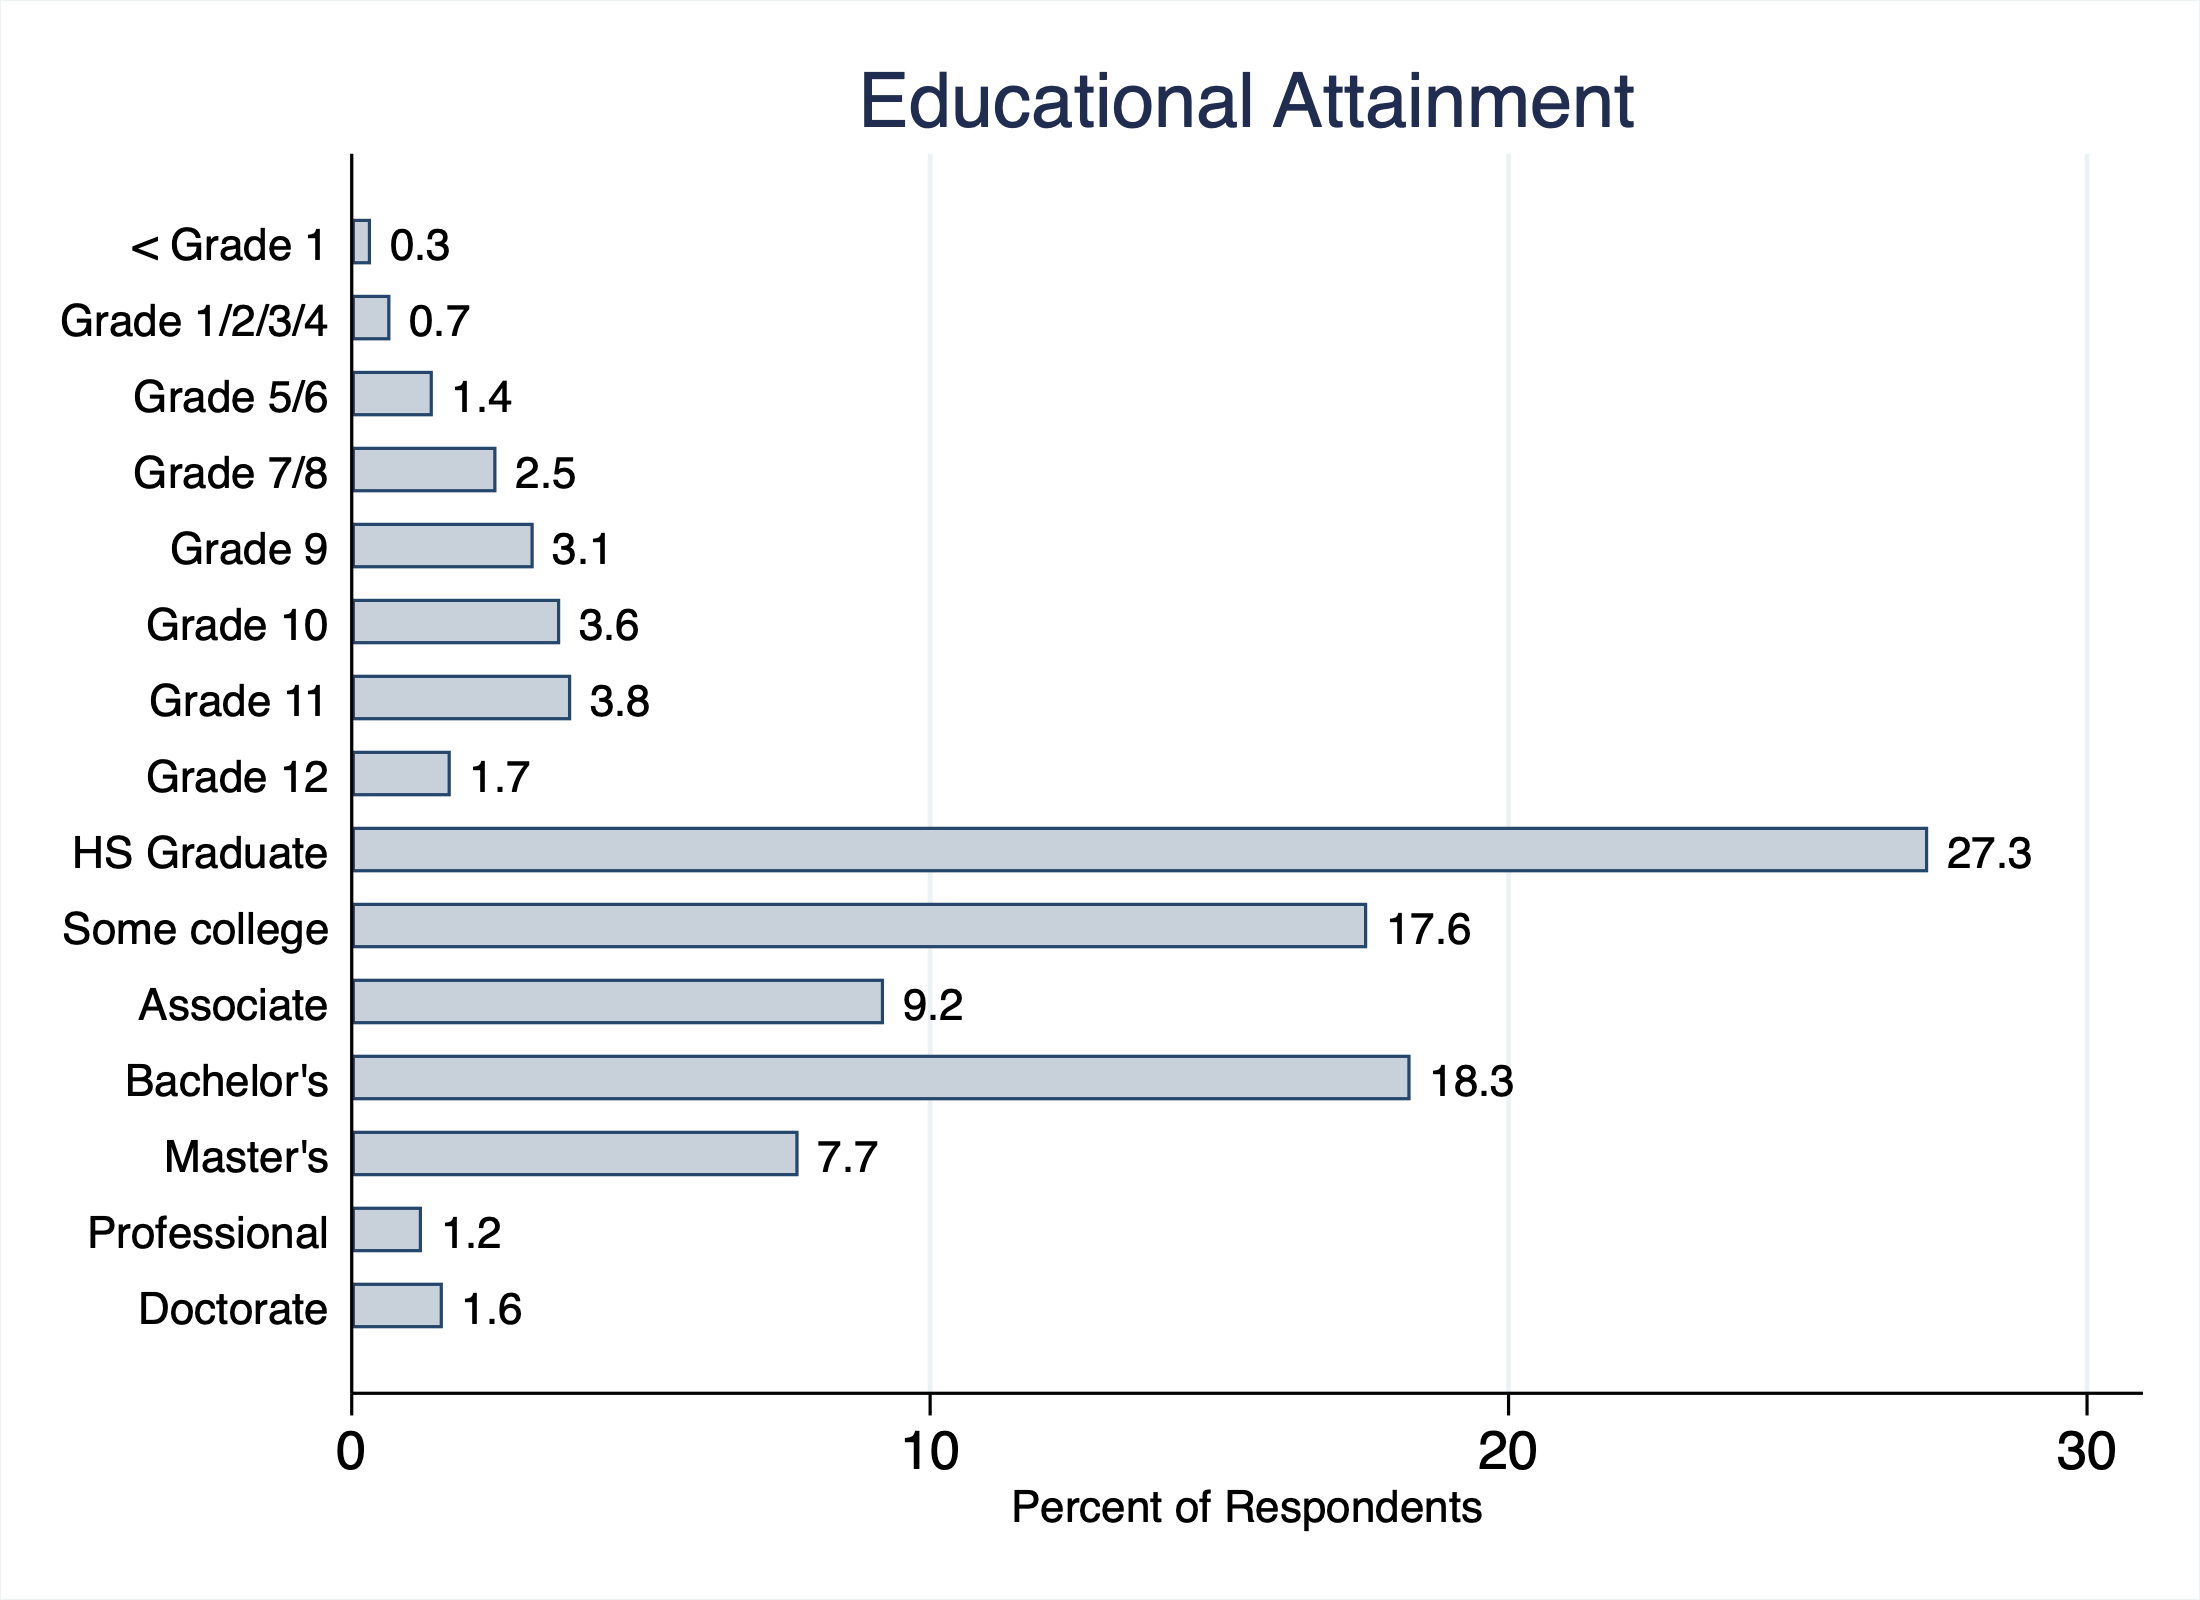
\includegraphics[width=8.5cm]{hist2.png}
	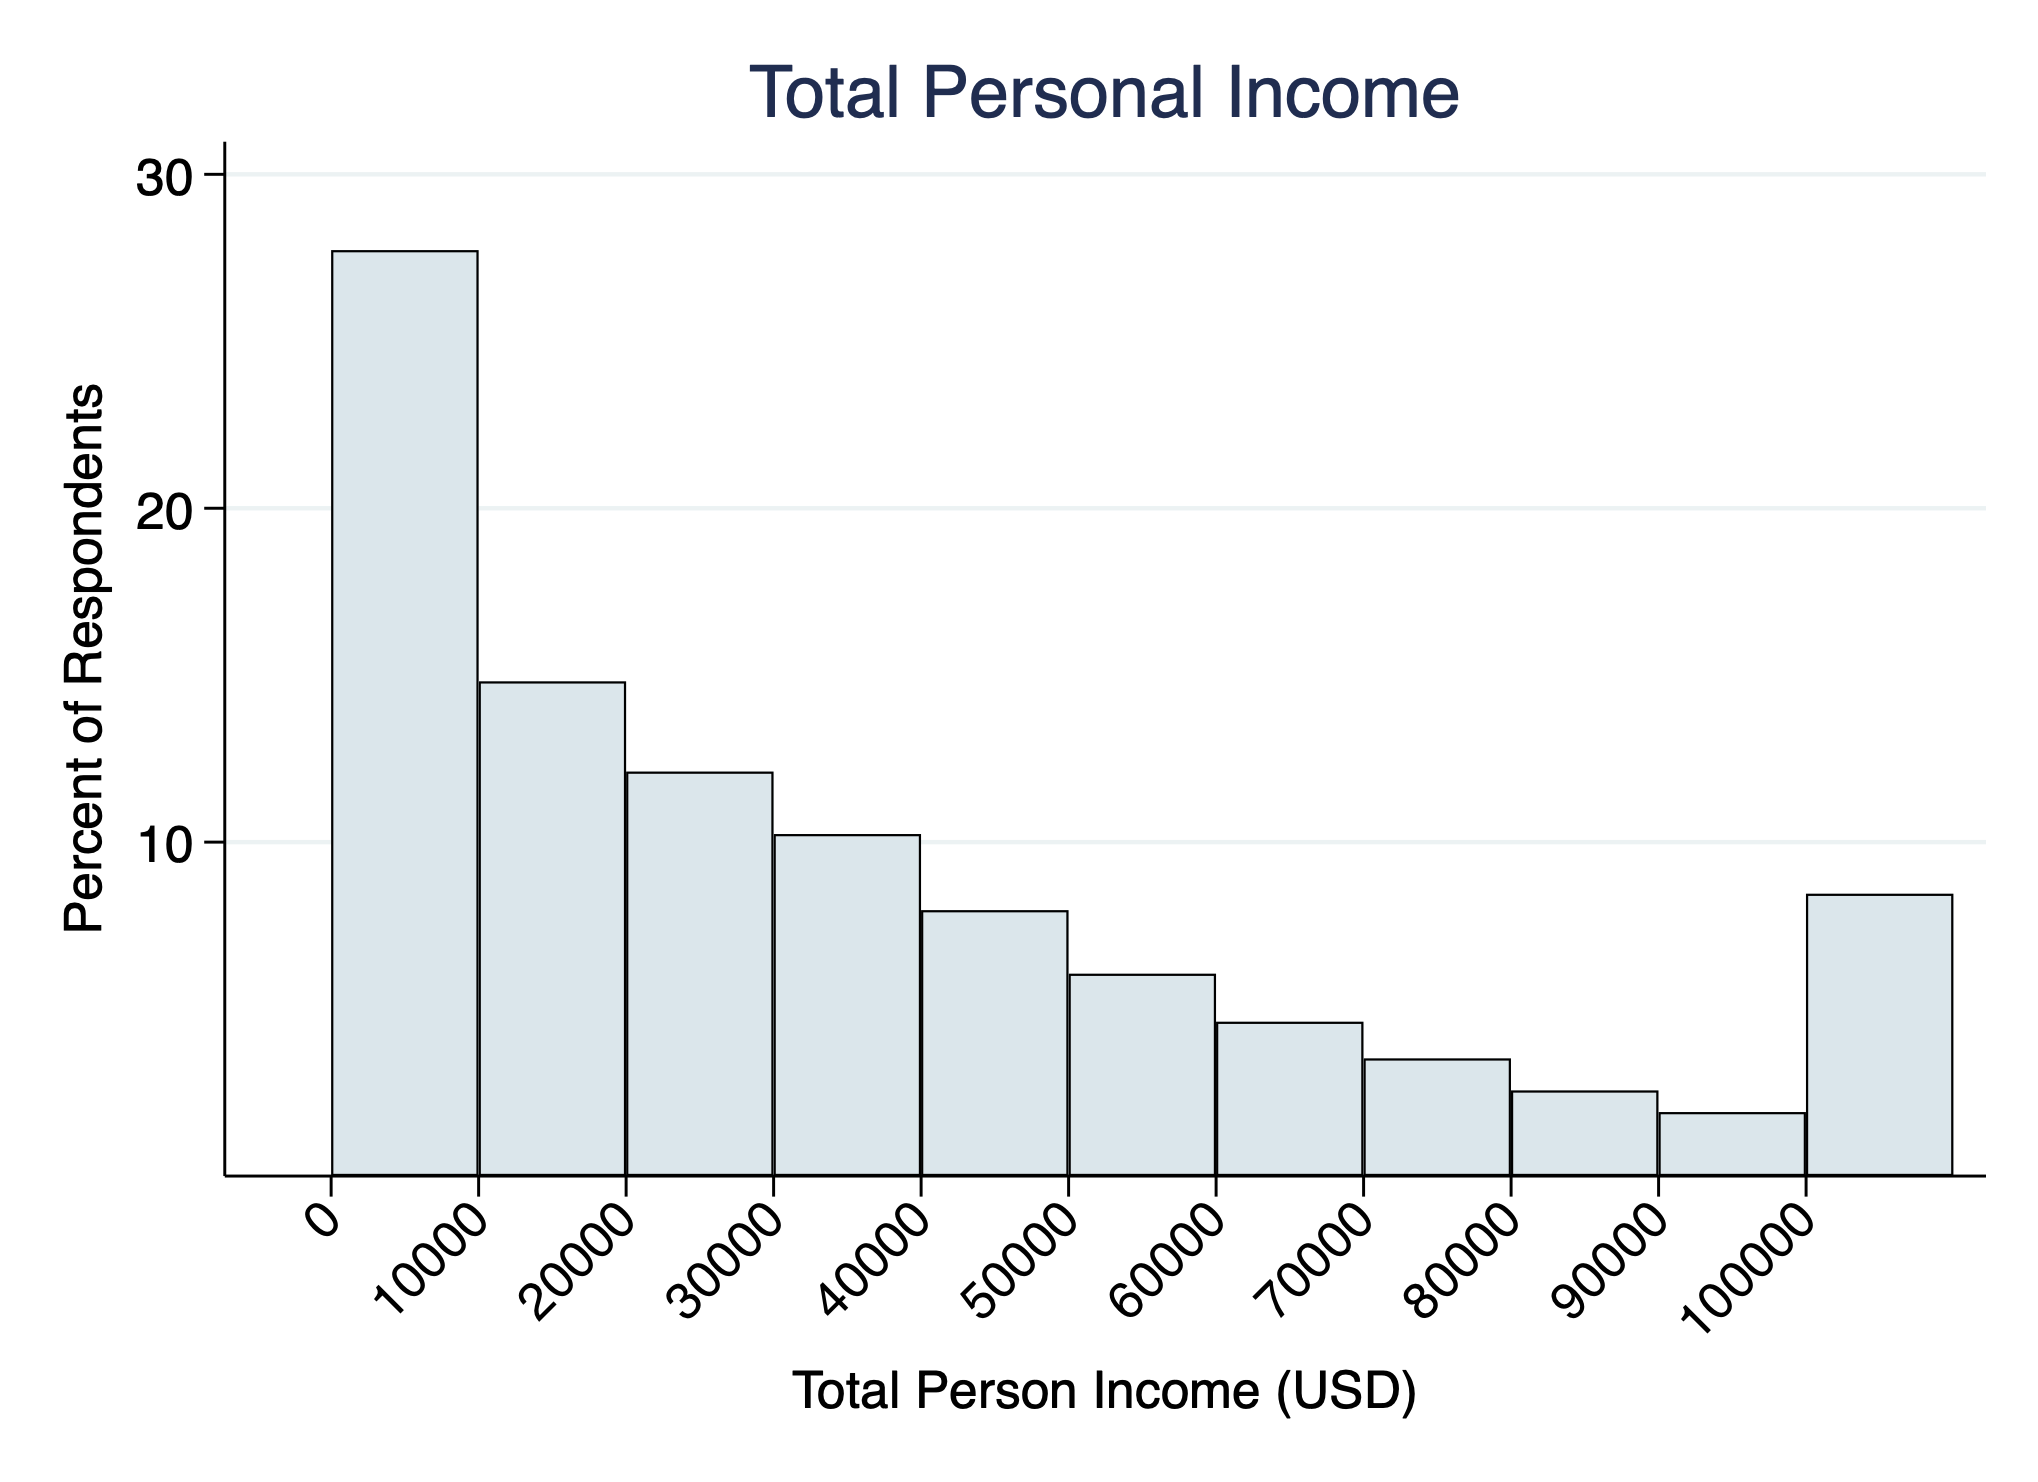
\includegraphics[width=8.5cm]{hist1.png}

\end{figure*}

These two figures, as well as the accompanying tabulated table in the appendix, describe the summary statistics. For both variables, the most interesting characteristic of the dataset is the distribution (i.e. relative frequency) across the variable. On the left, a bar chart is used, with each additional level of educational attainment being an additional bar on an ordinal trajectory, in order to preserve a roughly linear understanding of each 'step'. As for personal income, there are two things to be noted: A histogram is used in order to undo the topcoding of the underlying variable and resume the understanding of income as a continuous, rather than discrete measure. The width of each bin is set to 10000 in order to more easily discern the power-law distribution of income.\footnote{\#descriptivestats: For both educational attainment and income, I choose an appropriate statistic (relative income), justifying my choice (it explains the underlying distribution best), and --for the income variable-- create a histogram in order to convert income from a categorical variable back to a continuous one , and explain why bins of width 10000 were chosen (to reduce smaller granularity and display the power law distribution of income).} \\


\newgeometry{left=2cm, right=2cm, top=2cm}

Though both variables are coded as categorical, the underlying variables has interval properties, and it is possible (for the purposes of regression and hypothesis testing) to transform them onto a continuous scale with a few assumptions - by approximating with educational attainment with a `years in education' variable, corresponding to average and recommended ages for each educational stage, and by rounding up each income level to the nearest \$2,500 and by treating incomes above \$100,000 as equivalent. (See Appendix)\\

According to Pearl's interpretation of causality, an event (e.g. a rise in incomes) is considered to causally depend on a cause (e.g. educational attainment) if and only if, if the cause occurs then the event would have occured, and if the cause did not occur then the event would not have occured. Thus while an association (i.e. correlation) between educational attainment and income can clearly be observed --such as in Figure 2-- causality cannot be established without adjusting for selection bias: something not possible in cross-sectional data. It is possible, for example, that those who chose to pursue a Master's degree would make less, just as much, or even more money had they dropped out of high school, and vice versa.\footnote{\#causaleffect: I explain what a causal relationship is, explain it within the context of the research question while providing relevant examples, evaluate why it is not possible to elicit causal relationships with cross-sectional regression, and justifying it by referring to Judea Pearl's definition of causality.}\\



While causality cannot be determined, we can test if two groups have the same population mean for a single variable. Suppose we want to determine if there is a difference in personal income between those who graduated high school, and those who completed some portion of Grade 12 but did not receive a diploma (e.g. dropouts). Following the 5 components, we would determine this as follows:

\begin{enumerate}
\item \textbf{Determine the null and alternative hypotheses:} \\
Letting $\mu_G$ be the mean income of 12th graders who graduated, and $\mu_U$ of those who did not, we have:
$$ H_0: \mu_{G} - \mu_{U} = 0 \qquad H_A:\mu_G-\mu_U \neq 0$$
\item \textbf{Specify the test statistic and its distribution if the null hypothesis is true:} \\
An appropriate test is Welch's $t$. Like the Student's $t$-test, the Welch's $t$-test assumes normality of data within each group (and follows a similar $t$-distribution), but allows for unequal variance between between groups, as is the case. A quick look at the table in the appendix will show the normality assumption to be violated (there is considerable right skew among each level of educational attainment), however the Welch's $t$-test remains robust for skewed distributions and large sample sizes, as is the case. Thus the test statistic $t$ is robust.

\item \textbf{Select $\alpha$ and determine the rejection region:}\\
Here I choose a significance level of  $\alpha = 0.005 \iff t= \pm2.807$, for multiple reasons: it reduces the false positive error rate (which, because of its policy implications, would be more damaging than a false negative), enhances reproducibility (as opposed to $\alpha = 0.05 \iff t = \pm 1.96$), and, in order to maintain statistical power, demands a larger sample size (of which we have plenty).

\item \textbf{Calculate the sample value of the test statistic:}\\
The t-statistic, and degrees of freedom are, respectively:
$$ t = \frac{\bar{X}_1 - \bar{X}_2}{\sqrt{ \frac{s^2_1}{N_1} + \frac{s^2}{N_2}}} = 25.8317 \qquad v = \frac{ \big( \frac{s^2_1}{N_1} + \frac{s^2_2}{N_2}\big)^2}{\frac{s^4_1}{N^2_1 (N_1-1)} + \frac{s^4_2}{N^2_2 (N_2 - 1)}} = 2939.2$$
\item \textbf{State your conclusion:}\\
Since $t = 25.8317 > 2.807$, we can reject the null hypothesis at the $\alpha = 0.005$ significance level and conclude that $\mu_G \neq  \mu_U$. Furthermore, because a two-tailed test splits the significance and applies it in both directions, a more powerful one-tailed test will also yield significance, so $t=25.8317>2.576 \Rightarrow \mu_G > \mu_U$.\footnote{\#statisticalinference: I define the hypotheses, choose Welch's $t$-test and justify my choice by noting unequal variances, visually evaluate the non-normality of the income data and justify it by referring to the large sample size, appropriately use $t$-statistics to support my argument in a detailed and sophisticated way.} \\Further analyses are available in the appendix, and Stata code is given in the accompanying file.
\end{enumerate}
\\

Word Count: 800
\begin{landscape}

\thispagestyle{mylandscape}




\begin{table}[h]
\section*{Appendix}
\subsection*{Tabulated Income by Educational Attainment}
\begin{tabular}{|l|lllllllllllllll|l|}
\hline
\textbf{Income}    & \multicolumn{1}{l|}{\textit{\textless G1}} & \multicolumn{1}{l|}{\textit{G1-4}} & \multicolumn{1}{l|}{\textit{G5/6}} & \multicolumn{1}{l|}{\textit{G7/8}} & \multicolumn{1}{l|}{\textit{G9}} & \multicolumn{1}{l|}{\textit{G10}} & \multicolumn{1}{l|}{\textit{G11}} & \multicolumn{1}{l|}{\textit{G12}} & \multicolumn{1}{l|}{\textit{HS}} & \multicolumn{1}{l|}{\textit{College}} & \multicolumn{1}{l|}{\textit{AA}} & \multicolumn{1}{l|}{\textit{BA}} & \multicolumn{1}{l|}{\textit{MA}} & \multicolumn{1}{l|}{\textit{Prof.}} & \textit{PhD} & Total   \\ \hline
\$0--\$9,999       & 259                                        & 405                                 & 800                                & 2,215                              & 3,261                            & 3,734                             & 3,683                             & 1,286                             & 10,332                           & 6,665                                 & 2,276                            & 3,732                            & 1,151                            & 147                                 & 159          & 40,105  \\ \cline{1-1} \cline{17-17} 
\$10K--\$19,999 & 116                                        & 270                                 & 535                                & 654                                & 551                              & 668                               & 791                               & 429                               & 7,857                            & 4,519                                 & 1,887                            & 2,313                            & 672                              & 64                                  & 102          & 21,428  \\ \cline{1-1} \cline{17-17} 
\$20K--\$29,999 & 57                                         & 137                                 & 313                                & 327                                & 310                              & 361                               & 419                               & 275                               & 6,467                            & 3,612                                 & 1,896                            & 2,463                            & 662                              & 91                                  & 129          & 17,519  \\ \cline{1-1} \cline{17-17} 
\$30K--\$39,999 & 26                                         & 76                                  & 206                                & 160                                & 197                              & 186                               & 257                               & 177                               & 4,923                            & 3,139                                 & 1,880                            & 2,658                            & 744                              & 80                                  & 104          & 14,813  \\ \cline{1-1} \cline{17-17} 
\$40K--\$49,999 & 8                                          & 32                                  & 74                                 & 112                                & 95                               & 105                               & 163                               & 110                               & 3,246                            & 2,150                                 & 1,456                            & 2,772                            & 984                              & 95                                  & 115          & 11,517  \\ \cline{1-1} \cline{17-17} 
\$50K--\$59,999 & 8                                          & 18                                  & 35                                 & 57                                 & 43                               & 48                                & 66                                & 84                                & 2,221                            & 1,471                                 & 1,051                            & 2,292                            & 1,099                            & 134                                 & 138          & 8,765   \\ \cline{1-1} \cline{17-17} 
\$60K--\$69,999 & 0                                          & 15                                  & 25                                 & 32                                 & 25                               & 36                                & 40                                & 35                                & 1,363                            & 1,096                                 & 812                              & 1,984                            & 985                              & 90                                  & 148          & 6,686   \\ \cline{1-1} \cline{17-17} 
\$70K--\$79,999 & 4                                          & 3                                   & 10                                 & 15                                 & 23                               & 29                                & 26                                & 22                                & 915                              & 747                                   & 625                              & 1,598                            & 863                              & 65                                  & 153          & 5,098   \\ \cline{1-1} \cline{17-17} 
\$80K--\$89,999 & 0                                          & 5                                   & 7                                  & 11                                 & 10                               & 13                                & 12                                & 20                                & 609                              & 468                                   & 373                              & 1,243                            & 731                              & 85                                  & 121          & 3,708   \\ \cline{1-1} \cline{17-17} 
\$90K-\$99,999 & 2                                          & 0                                   & 5                                  & 8                                  & 7                                & 6                                 & 14                                & 12                                & 353                              & 361                                   & 283                              & 986                              & 534                              & 71                                  & 129          & 2,771   \\ \cline{1-1} \cline{17-17} 
\$100K and up   & 3                                          & 7                                   & 19                                 & 29                                 & 28                               & 27                                & 17                                & 28                                & 1,133                            & 1,165                                 & 773                              & 4,435                            & 2,748                            & 836                                 & 982          & 12,230  \\ \hline
Total              & \multicolumn{1}{l|}{483}                   & \multicolumn{1}{l|}{968}            & \multicolumn{1}{l|}{2,029}         & \multicolumn{1}{l|}{3,620}         & \multicolumn{1}{l|}{4,550}       & \multicolumn{1}{l|}{5,213}        & \multicolumn{1}{l|}{5,488}        & \multicolumn{1}{l|}{2,478}        & \multicolumn{1}{l|}{39,419}      & \multicolumn{1}{l|}{25,393}           & \multicolumn{1}{l|}{13,312}      & \multicolumn{1}{l|}{26,476}      & \multicolumn{1}{l|}{11,173}      & \multicolumn{1}{l|}{1,758}          & 2,280        & 144,640 \\ \hline
\end{tabular}
\end{table}

\end{landscape}

\subsection*{Regression of Years in Educational Attainment on Personal Income}

The following encodes educational attainment as a factor variable, and income as rounded up to the nearest \$2500, with a reasonable adjusted $R^2$ of 0.2479.
\begin{verbatim}
regress income i.a_hga

      Source |       SS           df       MS      Number of obs   =   144,640
-------------+----------------------------------   F(14, 144625)   =   3406.22
       Model |  3.5400e+13        14  2.5286e+12   Prob > F        =    0.0000
    Residual |  1.0736e+14   144,625   742340825   R-squared       =    0.2480
-------------+----------------------------------   Adj R-squared   =    0.2479
       Total |  1.4276e+14   144,639   987016611   Root MSE        =     27246

--------------------------------------------------------------------------------
        income |      Coef.   Std. Err.      t    P>|t|     [95% Conf. Interval]
---------------+----------------------------------------------------------------
         a_hga |
Grade 1/2/3/4  |    3407.92   1517.834     2.25   0.025      432.996    6382.844
    Grade 5/6  |   4463.417   1379.421     3.24   0.001     1759.779    7167.056
    Grade 7/8  |  -1005.997    1319.85    -0.76   0.446    -3592.877    1580.883
      Grade 9  |  -3615.122   1303.875    -2.77   0.006    -6170.691   -1059.553
     Grade 10  |  -3633.383   1295.893    -2.80   0.005    -6173.308   -1093.457
     Grade 11  |   -2365.24   1293.137    -1.83   0.067    -4899.763    169.2839
     Grade 12  |   3556.515   1355.179     2.62   0.009     900.3905    6212.639
  HS Graduate  |   14684.92   1247.305    11.77   0.000     12240.22    17129.61
 Some college  |   17509.91   1251.468    13.99   0.000     15057.06    19962.77
    Associate  |   24716.06   1262.023    19.58   0.000     22242.52     27189.6
   Bachelor's  |      37447    1250.99    29.93   0.000     34995.08    39898.91
     Master's  |    47538.6   1266.246    37.54   0.000     45056.78    50020.41
 Professional  |   59094.78   1399.715    42.22   0.000     56351.36    61838.19
    Doctorate  |   58905.82   1364.744    43.16   0.000     56230.95    61580.69
               |
         _cons |   11816.77   1239.733     9.53   0.000     9386.918    14246.62
--------------------------------------------------------------------------------	
\end{verbatim}

The following regression replaces educational attainment with an approximate figure of how many years of education one is expected to have undergone at each level of educational attainment

\begin{verbatim}
	      Source |       SS           df       MS      Number of obs   =   144,640
-------------+----------------------------------   F(1, 144638)    =  37812.21
       Model |  2.9587e+13         1  2.9587e+13   Prob > F        =    0.0000
    Residual |  1.1317e+14   144,638   782466066   R-squared       =    0.2072
-------------+----------------------------------   Adj R-squared   =    0.2072
       Total |  1.4276e+14   144,639   987016611   Root MSE        =     27973

--------------------------------------------------------------------------------
        income |      Coef.   Std. Err.      t    P>|t|     [95% Conf. Interval]
---------------+----------------------------------------------------------------
years_educated |   4443.184   22.84958   194.45   0.000     4398.399    4487.969
         _cons |  -27244.95   331.5916   -82.16   0.000    -27894.86   -26595.04
--------------------------------------------------------------------------------
\end{verbatim}

Overall, educational attainment seems to be a significant predictor of the variability in personal income. An interesting pattern is the negative correlation between Grade 7/8, 9, 10 and 11 on income. 

\subsection*{Regression of Educational Attainment and Age on Personal Income}
The CPS Survey data contains the variable $age1$, which discretizes the age of individuals, given as follows:
\begin{verbatim}
	     Age recode - |
Persons 15+ years |      Freq.     Percent        Cum.
------------------+-----------------------------------
         15 years |      2,954        2.04        2.04
  16 and 17 years |      5,936        4.10        6.15
  18 and 19 years |      4,789        3.31        9.46
  20 and 21 years |      4,198        2.90       12.36
   22 to 24 years |      6,407        4.43       16.79
   25 to 29 years |     11,325        7.83       24.62
   30 to 34 years |     12,549        8.68       33.30
   35 to 39 years |     13,380        9.25       42.55
   40 to 44 years |     12,233        8.46       51.00
   45 to 49 years |     12,383        8.56       59.56
   50 to 54 years |     12,040        8.32       67.89
   55 to 59 years |     11,449        7.92       75.80
   60 to 61 years |      4,248        2.94       78.74
   62 to 64 years |      5,821        4.02       82.77
   65 to 69 years |      8,568        5.92       88.69
   70 to 74 years |      6,431        4.45       93.14
75 years and over |      9,929        6.86      100.00
------------------+-----------------------------------
            Total |    144,640      100.00
\end{verbatim}

By recoding age as a continuous variable (e.g. individuals in the 62-64 year old category are considered 63), age can be included into the regression model to marginally increase the adjusted $R^2$.

\begin{verbatim}
      Source |       SS           df       MS      Number of obs   =   144,640
-------------+----------------------------------   F(15, 144624)   =   3355.85
       Model |  3.6860e+13        15  2.4573e+12   Prob > F        =    0.0000
    Residual |  1.0590e+14   144,624   732251692   R-squared       =    0.2582
-------------+----------------------------------   Adj R-squared   =    0.2581
       Total |  1.4276e+14   144,639   987016611   Root MSE        =     27060

--------------------------------------------------------------------------------
        income |      Coef.   Std. Err.      t    P>|t|     [95% Conf. Interval]
---------------+----------------------------------------------------------------
         a_hga |
Grade 1/2/3/4  |   2863.909   1507.533     1.90   0.057     -90.8264    5818.644
    Grade 5/6  |   4412.581   1370.016     3.22   0.001     1727.377    7097.785
    Grade 7/8  |   1348.493    1311.91     1.03   0.304    -1222.826    3919.812
      Grade 9  |   246.1911   1297.868     0.19   0.850    -2297.605    2789.987
     Grade 10  |   209.1666   1289.931     0.16   0.871    -2319.073    2737.406
     Grade 11  |    1342.36   1287.001     1.04   0.297    -1180.137    3864.857
     Grade 12  |   6102.091   1347.145     4.53   0.000     3461.712    8742.469
  HS Graduate  |   15518.72   1238.941    12.53   0.000     13090.42    17947.02
 Some college  |   19201.67   1243.512    15.44   0.000     16764.41    21638.93
    Associate  |   25723.61   1253.621    20.52   0.000     23266.54    28180.68
   Bachelor's  |   38549.01   1242.705    31.02   0.000     36113.33    40984.68
     Master's  |   48157.24   1257.688    38.29   0.000      45692.2    50622.28
 Professional  |   59447.86   1390.193    42.76   0.000     56723.11    62172.61
    Doctorate  |   59223.44   1355.457    43.69   0.000     56566.77     61880.1
               |
           age |   185.8119   4.161463    44.65   0.000     177.6555    193.9683
         _cons |   2160.516   1250.127     1.73   0.084    -289.7091    4610.741
--------------------------------------------------------------------------------
\end{verbatim}



\end{document}